\documentclass[portrait]{seminar}
%\usepackage{pandora}
\usepackage{color}
\usepackage{fancybox}
\usepackage{alltt}
\usepackage{epsfig}
\usepackage{rail}
\usepackage{bar}
\usepackage{url}
\usepackage{rotating}
\usepackage[normalem]{ulem}
\usepackage{latexsym}
\usepackage{amsmath}

\begin{document}

\boldmath
\newcommand{\RA}{$\rightarrow$}
\newcommand{\LL}{\mbox{$[$\hspace{-0.15em}$[$}}
\newcommand{\RR}{\mbox{$]$\hspace{-0.15em}$]$}}
\newcommand{\CC}[1]{\mbox{\tt $\LL$#1$\RR$}}

\slideframe{shadow}

%%% Activate one of these to get either Aarhus style or McGill style 
%%% by putting a #1 in the appropriate line.
\newcommand{\mcgill}[1]{#1}
\newcommand{\aarhus}[1]{}

%%% Define this to be the name of your term
\newcommand{\courseterm}{Fall 2012}




\aarhus{
\newpagestyle{dOvsstyle}{dOvs \courseterm Week 36 \hfil Introduction}{\hfil \thepage}
}

\mcgill{
\newpagestyle{dOvsstyle}{COMP 520 \courseterm  \hfil Introduction (\thepage)}{}
}
 
\slidepagestyle{dOvsstyle}

\begin{slide*}
\begin{tabbing}
\aarhus{ {\Large\bf Week 36}\\ }

~\\
{\Huge\bf Introduction}\\~\\
\mcgill{
COMP 520: Compiler Design \\
 Ismail Badawi \\
TRF 4:35-5:25 ENGTR 0060 \\
}
\end{tabbing}

\begin{center}
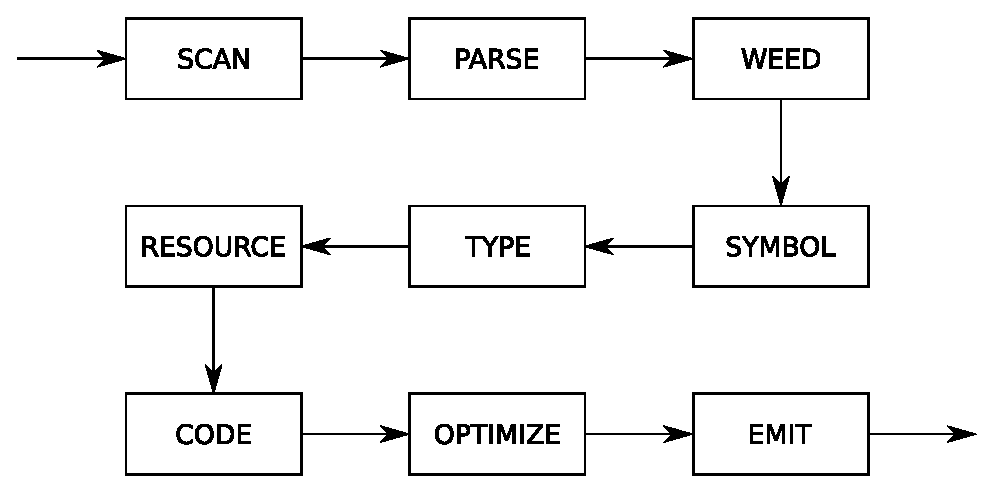
\psfig{file=figs/compiler_overview.eps,width=20em}
\end{center}
\end{slide*}

\begin{slide*}
Purpose:
\begin{itemize}
\item This course covers modern compiler techniques and their application to both
general-purpose and domain-specific languages.

\item The practical aspects focus on current technologies, primarily
  Java and interactive web services.
\end{itemize}
\vfil
\end{slide*}
 
\begin{slide*}
Contents:
\begin{itemize}\itemsep=0mm
\item {\em Deterministic parsing:\/} Scanners, LR parsers, the {\tt flex}/{\tt
  bison} and {\tt SableCC} tools.
\item {\em Semantic analysis:\/} abstract syntax trees, symbol tables \&
attribute grammars, type checking, resource allocation.
\item {\em Virtual machines and run-time environments:\/} stacks, heaps, objects.
\item {\em Code generation:\/} resources, templates, optimizations.
\item {\em Surveys on:\/} native code generation, static analysis, \ldots.
\end{itemize}
\vfil
\end{slide*}
 
\begin{slide*}
Schedule:
\begin{itemize}\itemsep=0mm
\item Lectures: 3 hours/week.
\aarhus{ \item {\em Tutorials:\/} 3 hours/week.  
         \item {\em Project:\/}   approx. 8 weeks. 
}
\end{itemize}

Prerequisites:
\begin{itemize}\itemsep=0mm
\aarhus{ 
\item Datalogi 1, Architecture (dArk), and Fundamental Models (dFM).
}
\mcgill{ 
\item COMP 273, COMP 302, (COMP 330), ability to read and write ``large'' programs.   

\item Students without COMP 330 should read the background material indicated
in Week 1 of the web page ASAP.
}
\end{itemize}

\aarhus{
Exam:
\begin{itemize}\itemsep=0mm
\item Oral exam based on the project work. The project evaluation will be included
               in the final grade.
\end{itemize}
}

\mcgill{
Lecturer:
\begin{itemize}\itemsep=0mm
\item Ismail Badawi, McConnell 226/234,
	\\Office hours TBD 
\end{itemize}
}

\mcgill{
TA:
\begin{itemize}\itemsep=0mm
\item Vineet Kumar, McConnell 226/234,\\
	Office Hours TBD
\end{itemize}
Midterm: in-class, near end of October\\
Final exam: during the final exam period, date TBA 
}

\vfil
\end{slide*}
 
\mcgill{
\begin{slide*}
Marking Scheme:
\begin{itemize}\itemsep=0mm
\item 10\% midterm, 25\% final exam, 65\% assignments and project
\item the 65\% for assignments and projects will be divided as follows: 
\begin{itemize}
\item 10\% for the first 3 JOOS deliverables (3.33\% each)
\item 10\% for the JOOS peephole optimizer
\item 25\% for content submitted at milestones
\item 20\% for the final WIG compiler and report
\end{itemize}
\item Group members may be given different grades on the project work if
the contributions are not reasonably equal.
% \item You have three late days for the term. Late days can be taken
% at any deadline \emph{but not at the final one}. 
\end{itemize}
\vfil
\end{slide*}
}

\mcgill{
\begin{slide*}
Academic Integrity:
\begin{itemize}
\item McGill University values academic integrity. Therefore all
  students must understand the meaning and consequences of cheating,
  plagiarism and other academic offences under the Code of Student
  Conduct and Disciplinary Procedures.\\
  {\footnotesize \url{http://www.mcgill.ca/integrity/studentguide/}}

\item In terms of this course, part of your responsibility is to
  ensure that you put the name of the author on all code that is
  submitted.  By putting your name on the code you are indicating that
  it is completely your own work.

\item If you use some third-party code you
  must have permission to use it and you must clearly indicate the
  source of the code.
\end{itemize}
\vfil
\end{slide*}
}

\begin{slide*}
Course material:
\begin{itemize}
\item course pack readings (readings C1-C8);
\item online readings (readings O1-O5);
\item slides for the lectures; and
\item extensive documentation on the course web pages.
\end{itemize}
\vfil
\end{slide*}

\begin{slide*}
The course pack and the online readings:
\begin{itemize}
\item are mainly background reading;
\item do not discuss the JOOS and WIG projects used in this course; and
\item are required for the exercises.
\end{itemize}
The slides:
\begin{itemize}
\item are quite detailed; and
\aarhus{
\item will be printed at the end of the course.
}
\mcgill{
% \item will be available at the EUS Copy Center in McConnell by the
% beginning of the second week of lectures.
\item are available online just before class in 1-up and 4-up formats.
}
\end{itemize}
The web pages:
\begin{itemize}
\item aim to contain all information;
\item provide on-line documentation; and
\item may be updated frequently.
\end{itemize}
\vfil
\end{slide*}

% \begin{slide*}
% New this year: The newsgroup {\small 
% \url{http://groups.google.com/group/comp-520-08}}

% \begin{itemize}
% \item Restricted to COMP 520 students, TA and the instructor
% \begin{itemize}
%   \item Visit group and ask for an invitation to join
%   \item We will then approve your invitation
% \end{itemize} 
% \item Main purpose is to discuss:
% \begin{itemize}
%   \item Problems you may encounter with the tools you need to use, and
%   \item Questions about the previous lecture(s)
% \end{itemize}
% \item Do \emph{not} use this group for:
% \begin{itemize}
%   \item Questions regarding solutions to exercises, assignments or your
%   projects (see/email the TA instead)
%   \item Anything personal, etc. (see TA or instructor)
% \end{itemize} 
% \end{itemize} 
% \end{slide*}

\begin{slide*}
Subversion (SVN)

\begin{itemize}
\item Versioning system
\item Good for maintaining source code but also for other things
\item You will use it for your submissions
\item You can also use it to track changes on the website and to access your
source code templates
\item Tasks for this week
	\begin{itemize}
      \item Read SVN documentation on the website
      \item Pair up with group mates (may use discussion group)
      \item Send SSH key and name(s) of group mate(s) to the TA (see website) 
	\end{itemize}
\end{itemize} 
\vfill
\end{slide*}

 
\begin{slide*}
New programming languages per year:\\

\begin{barenv}
\setnumberpos{empty}
\setwidth{9}
\setstyle{\scriptsize}
\setxaxis{52}{72}{1}
\setyaxis{0}{100}{10}
\bar{3}{1}
\bar{2}{1}
\bar{2}{1}
\bar{1}{1}
\bar{1}{8}
\bar{9}{1}
\bar{14}{1}
\bar{99}{1}
\bar{23}{1}
\bar{21}{1}
\bar{19}{1}
\bar{18}{1}
\bar{31}{1}
\bar{32}{1}
\bar{45}{1}
\bar{35}{1}
\bar{53}{1}
\bar{58}{1}
\bar{60}{1}
\bar{54}{1}
\bar{39}{1}
\end{barenv}
\vspace{8mm}
\begin{barenv}
\setnumberpos{empty}
\setwidth{9}
\setstyle{\scriptsize}
\setxaxis{73}{93}{1}
\setyaxis{0}{130}{10}
\bar{40}{1}
\bar{47}{1}
\bar{56}{1}
\bar{54}{1}
\bar{59}{1}
\bar{71}{1}
\bar{56}{1}
\bar{76}{1}
\bar{51}{1}
\bar{62}{1}
\bar{59}{1}
\bar{77}{1}
\bar{82}{1}
\bar{126}{1}
\bar{109}{1}
\bar{99}{1}
\bar{112}{1}
\bar{113}{1}
\bar{96}{1}
\bar{65}{1}
\bar{55}{1}
\end{barenv}
\vfil
\end{slide*}

\begin{slide*}
The compiler for the FORTRAN language:
\begin{itemize}
\item was implemented in 1954--1957;
\item was the world's first compiler;
\item was motivated by the economics of programming;
\item had to overcome deep skepticism;
\item paid little attention to language design;
\item focused on efficiency of the generated code;
\item pioneered many concepts and techniques; and
\item revolutionized computer programming.
\end{itemize}
\vfil
\end{slide*}

\begin{slide*}
{\scriptsize
\begin{verbatim}
C AREA OF A TRIANGLE WITH A STANDARD SQUARE ROOT FUNCTION 
C INPUT - CARD READER UNIT 5, INTEGER INPUT
C OUTPUT - LINE PRINTER UNIT 6, REAL OUTPUT
C INPUT ERROR DISPLAY ERROR OUTPUT CODE 1 IN JOB CONTROL
  LISTING
      READ INPUT TAPE 5, 501, IA, IB, IC
  501 FORMAT (3I5)
C IA, IB, AND IC MAY NOT BE NEGATIVE
C FURTHERMORE, THE SUM OF TWO SIDES OF A TRIANGLE
C IS GREATER THAN THE THIRD SIDE, SO WE CHECK FOR THAT, TOO
      IF (IA) 777, 777, 701
  701 IF (IB) 777, 777, 702
  702 IF (IC) 777, 777, 703
  703 IF (IA+IB-IC) 777,777,704
  704 IF (IA+IC-IB) 777,777,705
  705 IF (IB+IC-IA) 777,777,799
  777 STOP 1
C USING HERON'S FORMULA WE CALCULATE THE
C AREA OF THE TRIANGLE
  799 S = FLOATF (IA + IB + IC) / 2.0
      AREA = SQRT( S * (S - FLOATF(IA)) * (S - FLOATF(IB)) *
     +     (S - FLOATF(IC)))
      WRITE OUTPUT TAPE 6, 601, IA, IB, IC, AREA
  601 FORMAT (4H A= ,I5,5H  B= ,I5,5H  C= ,I5,8H  AREA= ,
     F10.2, 
     +        13H SQUARE UNITS)
      STOP
      END 
\end{verbatim}
} 
\end{slide*}

\begin{slide*}
General-purpose languages:
\begin{itemize}
\item allow for arbitrarily useful programs to be written
\item in the theoretical sense are all Turing-complete; and
\item are the focus of most programming language courses.
\end{itemize}
Prominent examples are:
\begin{itemize}
\item C
\item C++
\item FORTRAN
\item Java
\item \ldots
\end{itemize}
General purpose languages fairly obviously require full-scale compiler
technology to run efficiently.
\vfil
\end{slide*}
 
\begin{slide*}
Domain-specific languages:
\begin{itemize}
\item extend software design; and
\item are concrete artifacts that permit representation, optimization, and analysis in ways
      that low-level programs and libraries do not.
\item They may even be visual! (e.g. boxes \& arrows) 
\end{itemize}
Prominent examples are:
\begin{itemize}
\item \LaTeX
\item {\tt yacc} and {\tt lex}
\item Makefiles
\item HTML
\item SVG
\item \ldots
\end{itemize}
Domain-specific languages also require full-scale compiler technology.
\vfil
\end{slide*}

\begin{slide*}
Reasons to learn compiler technology:
\begin{itemize}
\item understand existing languages;
\item appreciate current limitations;
\item talk intelligently about language design;
\item implement your very own general purpose language; and
\item implement lots of useful domain-specific languages
\begin{itemize}
\item encoding everything in XML is not always the best way to go\\
	(see Makefiles vs. Ant's build.xml)  
\end{itemize}
\end{itemize}
\vfil
\end{slide*}
 
\begin{slide*}
The phases of a modern compiler:\\

\begin{center}
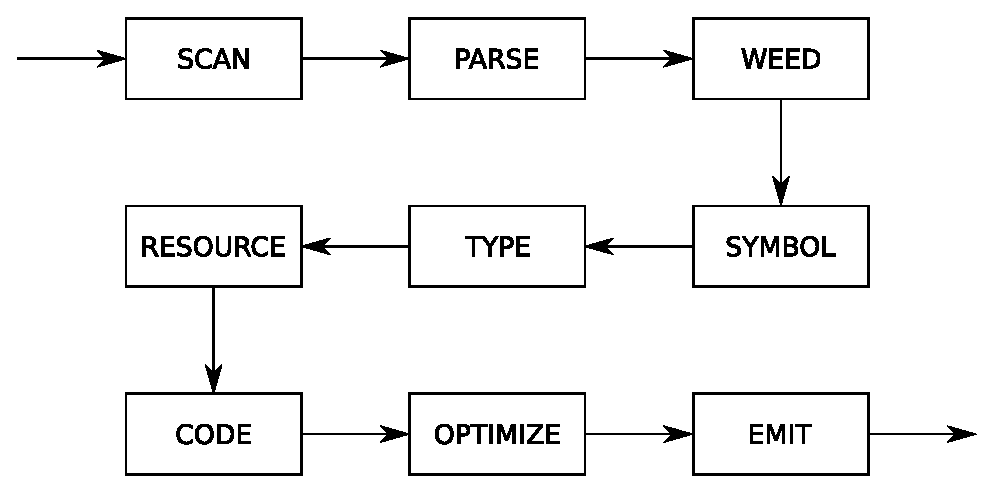
\psfig{file=figs/compiler_overview.eps,width=20em}
\end{center}

The individual phases:
\begin{itemize}
\item are modular software components;
\item have their own standard technology; and
\item are increasingly being supported by automatic tools.
\end{itemize}

Advanced backends may contain an additional 5--10 phases.
\vfil
\end{slide*}
 
\begin{slide*}
The 
\psfig{file=joos.EPSF,width=5em} project:
\begin{itemize}
\item \underline{J}ava's \underline{O}bject-\underline{O}riented \underline{S}ubset
\item is compiled to Java bytecode;
\item illustrates a general purpose language;
\item allows client-side programming on the web;
\item is used to teach by example;
\item has $\;$
\psfig{file=a-.eps,width=2em} source code available;
\item and will be upgraded by you into an $\;$
\psfig{file=a+.eps,width=2em} version.
\end{itemize}
\vfil
\end{slide*}
 
\begin{slide*}
The 
\psfig{file=wig.EPSF,width=5em} project:
\begin{itemize}
\item \underline{W}eb \underline{I}nterface \underline{G}enerator
\item is compiled to C-based CGI-scripts (or other targets...);
\item illustrates a domain-specific language;
\item allows server-side programming on the web;
\item is used to get hands-on experience;
\item and will be implemented from scratch, by you!
\end{itemize}
\vfil
\end{slide*}

\begin{slide*}
The top 10 list of reasons why we use C for compilers:\\

\begin{itemize}
\item[10)] it's tradition;
\item[9)] it's (truly) portable;
\item[8)] it's efficient;
\item[7)] it has many different uses;
\item[6)] ANSI C will never change;
\item[5)] you must learn C at some point;
\item[4)] it teaches discipline (the hard way);
\item[3)] methodology is language independent;
\item[2)] we have {\tt flex} and {\tt bison}; and
\item[1)] you can say that you have implemented a large project in C.
\end{itemize}
\vfil
\end{slide*}

\begin{slide*}
The top 10 list of reasons why we use Java for compilers:\\

\begin{small}
\begin{itemize}
\item[10)] you already know Java from previous courses;
\item[9)] run-time errors like null-pointer exceptions are easy to locate;
\item[8)] it is relatively strongly typed, so many errors are caught at compile
time;
\item[7)] you can use the large Java library (hash maps, sets, lists, \ldots);
\item[6)] Java bytecode is portable and can be executed without recompilation;
\item[5)] you don't mind slow compilers;
\item[4)] it allows you to use object-orientation;
\item[3)] methodology is language independent;
\item[2)] we have {\tt sablecc}, developed at McGill; and
\item[1)] you can say that you have implemented a large project in Java.
\end{itemize}
\vfil
\end{small}
\end{slide*}

\begin{slide*}
How to bootstrap a compiler (SCALA example):
 
\begin{itemize}
\item we are given a source language (L in the reading), say SCALA; and
\item a target language (M in the reading), say Java.
\end{itemize}
\vspace*{1em}

We need the following:\\

\begin{tabbing}
~~~~~~~~~~~
\setlength{\unitlength}{3947sp}%
%
\begingroup\makeatletter\ifx\SetFigFont\undefined%
\gdef\SetFigFont#1#2#3#4#5{%
  \reset@font\fontsize{#1}{#2pt}%
  \fontfamily{#3}\fontseries{#4}\fontshape{#5}%
  \selectfont}%
\fi\endgroup%
\begin{picture}(1650,891)(3301,-3040)
\thicklines
\put(3901,-2161){\line( 0,-1){300}}
\put(3901,-2461){\line( 1, 0){300}}
\put(4201,-2461){\line( 0,-1){300}}
\put(4201,-2761){\line( 1, 0){300}}
\put(4501,-2761){\line( 0, 1){300}}
\put(4501,-2461){\line( 1, 0){300}}
\put(4801,-2461){\line( 0, 1){300}}
\put(4801,-2161){\line(-1, 0){900}}
\put(3361,-2356){\makebox(0,0)[lb]{\smash{\SetFigFont{8}{14.4}{\familydefault}{\mddefault}{\updefault}source}}}
\put(4951,-2356){\makebox(0,0)[lb]{\smash{\SetFigFont{8}{14.4}{\familydefault}{\mddefault}{\updefault}target}}}
\put(3900,-2956){\makebox(0,0)[lb]{\smash{\SetFigFont{8}{14.4}{\familydefault}{\mddefault}{\updefault}implementation}}}
\put(3976,-2386){\makebox(0,0)[lb]{\smash{\SetFigFont{12}{14.4}{\familydefault}{\mddefault}{\updefault}S}}}
\put(4556,-2386){\makebox(0,0)[lb]{\smash{\SetFigFont{12}{14.4}{\familydefault}{\mddefault}{\updefault}J}}}
\put(4256,-2686){\makebox(0,0)[lb]{\smash{\SetFigFont{12}{14.4}{\familydefault}{\mddefault}{\updefault}J}}}
\end{picture}
\end{tabbing}

Of course, actually we like SCALA much better than Java and would therefore
rather implement SCALA in itself:\\

\begin{tabbing}
~~~~~~~~~~~
\setlength{\unitlength}{3947sp}%
%
\begingroup\makeatletter\ifx\SetFigFont\undefined%
\gdef\SetFigFont#1#2#3#4#5{%
  \reset@font\fontsize{#1}{#2pt}%
  \fontfamily{#3}\fontseries{#4}\fontshape{#5}%
  \selectfont}%
\fi\endgroup%
\begin{picture}(1650,891)(3301,-3040)
\thicklines
\put(3901,-2161){\line( 0,-1){300}}
\put(3901,-2461){\line( 1, 0){300}}
\put(4201,-2461){\line( 0,-1){300}}
\put(4201,-2761){\line( 1, 0){300}}
\put(4501,-2761){\line( 0, 1){300}}
\put(4501,-2461){\line( 1, 0){300}}
\put(4801,-2461){\line( 0, 1){300}}
\put(4801,-2161){\line(-1, 0){900}}
\put(3361,-2356){\makebox(0,0)[lb]{\smash{\SetFigFont{8}{14.4}{\familydefault}{\mddefault}{\updefault}source}}}
\put(4951,-2356){\makebox(0,0)[lb]{\smash{\SetFigFont{8}{14.4}{\familydefault}{\mddefault}{\updefault}target}}}
\put(3900,-2956){\makebox(0,0)[lb]{\smash{\SetFigFont{8}{14.4}{\familydefault}{\mddefault}{\updefault}implementation}}}
\put(3976,-2386){\makebox(0,0)[lb]{\smash{\SetFigFont{12}{14.4}{\familydefault}{\mddefault}{\updefault}S}}}
\put(4556,-2386){\makebox(0,0)[lb]{\smash{\SetFigFont{12}{14.4}{\familydefault}{\mddefault}{\updefault}J}}}
\put(4256,-2686){\makebox(0,0)[lb]{\smash{\SetFigFont{12}{14.4}{\familydefault}{\mddefault}{\updefault}S}}}
\end{picture}
\end{tabbing}
\vfil
\end{slide*}
 
\begin{slide*}
Define the following:
\begin{itemize}
\item S$^{\downarrow}$ is a simple subset of SCALA;
\item J$^-$ is inefficient Java code, and
\item P is our favourite programming language, here ``Pizza''. 
\end{itemize}
\vspace*{2em}

We can easily implement:
\begin{center}
\setlength{\unitlength}{3947sp}%
%
\begingroup\makeatletter\ifx\SetFigFont\undefined%
\gdef\SetFigFont#1#2#3#4#5{%
  \reset@font\fontsize{#1}{#2pt}%
  \fontfamily{#3}\fontseries{#4}\fontshape{#5}%
  \selectfont}%
\fi\endgroup%
\begin{picture}(924,624)(3889,-2773)
\thicklines
\put(3901,-2161){\line( 0,-1){300}}
\put(3901,-2461){\line( 1, 0){300}}
\put(4201,-2461){\line( 0,-1){300}}
\put(4201,-2761){\line( 1, 0){300}}
\put(4501,-2761){\line( 0, 1){300}}
\put(4501,-2461){\line( 1, 0){300}}
\put(4801,-2461){\line( 0, 1){300}}
\put(4801,-2161){\line(-1, 0){900}}
\put(3976,-2386){\makebox(0,0)[lb]{\smash{\SetFigFont{12}{14.4}{\familydefault}{\mddefault}{\updefault}S$^{\downarrow}$}}}
\put(4500,-2386){\makebox(0,0)[lb]{\smash{\SetFigFont{12}{14.4}{\familydefault}{\mddefault}{\updefault}J$^-$}}}
\put(4256,-2686){\makebox(0,0)[lb]{\smash{\SetFigFont{12}{14.4}{\familydefault}{\mddefault}{\updefault}P}}}
\put(4306,-2386){\makebox(0,0)[lb]{\smash{\SetFigFont{6}{14.4}{\familydefault}{\mddefault}{\updefault}1}}}
\end{picture}
\end{center}
and in parallel, using S$^{\downarrow}$, we can implement:
\begin{center}
\setlength{\unitlength}{3947sp}%
%
\begingroup\makeatletter\ifx\SetFigFont\undefined%
\gdef\SetFigFont#1#2#3#4#5{%
  \reset@font\fontsize{#1}{#2pt}%
  \fontfamily{#3}\fontseries{#4}\fontshape{#5}%
  \selectfont}%
\fi\endgroup%
\begin{picture}(924,624)(3889,-2773)
\thicklines
\put(3901,-2161){\line( 0,-1){300}}
\put(3901,-2461){\line( 1, 0){300}}
\put(4201,-2461){\line( 0,-1){300}}
\put(4201,-2761){\line( 1, 0){300}}
\put(4501,-2761){\line( 0, 1){300}}
\put(4501,-2461){\line( 1, 0){300}}
\put(4801,-2461){\line( 0, 1){300}}
\put(4801,-2161){\line(-1, 0){900}}
\put(3976,-2386){\makebox(0,0)[lb]{\smash{\SetFigFont{12}{14.4}{\familydefault}{\mddefault}{\updefault}S}}}
\put(4556,-2386){\makebox(0,0)[lb]{\smash{\SetFigFont{12}{14.4}{\familydefault}{\mddefault}{\updefault}J}}}
\put(4276,-2686){\makebox(0,0)[lb]{\smash{\SetFigFont{12}{14.4}{\familydefault}{\mddefault}{\updefault}S$^{\downarrow}$}}}
\put(4306,-2386){\makebox(0,0)[lb]{\smash{\SetFigFont{6}{14.4}{\familydefault}{\mddefault}{\updefault}2}}}
\end{picture}
\end{center}
using basically our favourite language.
\vfil
\end{slide*}
 
\begin{slide*}
Combining the two compilers, we get:\\

\begin{center}
\setlength{\unitlength}{3947sp}%
%
\begingroup\makeatletter\ifx\SetFigFont\undefined%
\gdef\SetFigFont#1#2#3#4#5{%
  \reset@font\fontsize{#1}{#2pt}%
  \fontfamily{#3}\fontseries{#4}\fontshape{#5}%
  \selectfont}%
\fi\endgroup%
\begin{picture}(2274,999)(3889,-3148)
\thinlines
\put(3901,-2161){\line( 0,-1){300}}
\put(3901,-2461){\line( 1, 0){300}}
\put(4201,-2461){\line( 0,-1){300}}
\put(4201,-2761){\line( 1, 0){300}}
\put(4501,-2761){\line( 0, 1){300}}
\put(4501,-2461){\line( 1, 0){300}}
\put(4801,-2461){\line( 0, 1){300}}
\put(4801,-2161){\line(-1, 0){900}}
\put(4576,-2536){\line( 0,-1){300}}
\put(4576,-2836){\line( 1, 0){300}}
\put(4876,-2836){\line( 0,-1){300}}
\put(4876,-3136){\line( 1, 0){300}}
\put(5176,-3136){\line( 0, 1){300}}
\put(5176,-2836){\line( 1, 0){300}}
\put(5476,-2836){\line( 0, 1){300}}
\put(5476,-2536){\line(-1, 0){900}}
\put(5251,-2161){\line( 0,-1){300}}
\put(5251,-2461){\line( 1, 0){300}}
\put(5551,-2461){\line( 0,-1){300}}
\put(5551,-2761){\line( 1, 0){300}}
\put(5851,-2761){\line( 0, 1){300}}
\put(5851,-2461){\line( 1, 0){300}}
\put(6151,-2461){\line( 0, 1){300}}
\put(6151,-2161){\line(-1, 0){900}}
\put(3976,-2386){\makebox(0,0)[lb]{\smash{\SetFigFont{12}{14.4}{\familydefault}{\mddefault}{\updefault}S}}}
\put(4556,-2386){\makebox(0,0)[lb]{\smash{\SetFigFont{12}{14.4}{\familydefault}{\mddefault}{\updefault}J}}}
\put(4276,-2686){\makebox(0,0)[lb]{\smash{\SetFigFont{12}{14.4}{\familydefault}{\mddefault}{\updefault}S$^{\downarrow}$}}}
\put(4306,-2386){\makebox(0,0)[lb]{\smash{\SetFigFont{6}{14.4}{\familydefault}{\mddefault}{\updefault}2}}}
\put(4651,-2761){\makebox(0,0)[lb]{\smash{\SetFigFont{12}{14.4}{\familydefault}{\mddefault}{\updefault}S$^{\downarrow}$}}}
\put(5161,-2761){\makebox(0,0)[lb]{\smash{\SetFigFont{12}{14.4}{\familydefault}{\mddefault}{\updefault}J$^-$}}}
\put(4931,-3061){\makebox(0,0)[lb]{\smash{\SetFigFont{12}{14.4}{\familydefault}{\mddefault}{\updefault}P}}}
\put(4971,-2761){\makebox(0,0)[lb]{\smash{\SetFigFont{6}{14.4}{\familydefault}{\mddefault}{\updefault}1}}}
\put(5326,-2386){\makebox(0,0)[lb]{\smash{\SetFigFont{12}{14.4}{\familydefault}{\mddefault}{\updefault}S}}}
\put(5906,-2386){\makebox(0,0)[lb]{\smash{\SetFigFont{12}{14.4}{\familydefault}{\mddefault}{\updefault}J}}}
\put(5596,-2686){\makebox(0,0)[lb]{\smash{\SetFigFont{12}{14.4}{\familydefault}{\mddefault}{\updefault}J$^-$}}}
\put(5666,-2386){\makebox(0,0)[lb]{\smash{\SetFigFont{6}{14.4}{\familydefault}{\mddefault}{\updefault}2'}}}
\end{picture}
\end{center}
which is an inefficient SCALA compiler (based on generated Java code) generating
efficient Java code.\\

A final combination gives us what we want:\\

\begin{center}
\setlength{\unitlength}{3947sp}%
%
\begingroup\makeatletter\ifx\SetFigFont\undefined%
\gdef\SetFigFont#1#2#3#4#5{%
  \reset@font\fontsize{#1}{#2pt}%
  \fontfamily{#3}\fontseries{#4}\fontshape{#5}%
  \selectfont}%
\fi\endgroup%
\begin{picture}(2949,1374)(3889,-3148)
\thinlines
\put(3901,-2161){\line( 0,-1){300}}
\put(3901,-2461){\line( 1, 0){300}}
\put(4201,-2461){\line( 0,-1){300}}
\put(4201,-2761){\line( 1, 0){300}}
\put(4501,-2761){\line( 0, 1){300}}
\put(4501,-2461){\line( 1, 0){300}}
\put(4801,-2461){\line( 0, 1){300}}
\put(4801,-2161){\line(-1, 0){900}}
\put(3976,-2386){\makebox(0,0)[lb]{\smash{\SetFigFont{12}{14.4}{\familydefault}{\mddefault}{\updefault}S}}}
\put(4556,-2386){\makebox(0,0)[lb]{\smash{\SetFigFont{12}{14.4}{\familydefault}{\mddefault}{\updefault}J}}}
\put(4276,-2686){\makebox(0,0)[lb]{\smash{\SetFigFont{12}{14.4}{\familydefault}{\mddefault}{\updefault}S$^{\downarrow}$}}}
\put(4326,-2386){\makebox(0,0)[lb]{\smash{\SetFigFont{6}{14.4}{\familydefault}{\mddefault}{\updefault}2}}}
\put(4576,-1786){\line( 0,-1){300}}
\put(4576,-2086){\line( 1, 0){300}}
\put(4876,-2086){\line( 0,-1){300}}
\put(4876,-2386){\line( 1, 0){300}}
\put(5176,-2386){\line( 0, 1){300}}
\put(5176,-2086){\line( 1, 0){300}}
\put(5476,-2086){\line( 0, 1){300}}
\put(5476,-1786){\line(-1, 0){900}}
\put(4651,-2011){\makebox(0,0)[lb]{\smash{\SetFigFont{12}{14.4}{\familydefault}{\mddefault}{\updefault}S}}}
\put(5231,-2011){\makebox(0,0)[lb]{\smash{\SetFigFont{12}{14.4}{\familydefault}{\mddefault}{\updefault}J}}}
\put(4951,-2311){\makebox(0,0)[lb]{\smash{\SetFigFont{12}{14.4}{\familydefault}{\mddefault}{\updefault}S}}}
\put(4981,-2011){\makebox(0,0)[lb]{\smash{\SetFigFont{6}{14.4}{\familydefault}{\mddefault}{\updefault}3}}}
\put(5926,-1786){\line( 0,-1){300}}
\put(5926,-2086){\line( 1, 0){300}}
\put(6226,-2086){\line( 0,-1){300}}
\put(6226,-2386){\line( 1, 0){300}}
\put(6526,-2386){\line( 0, 1){300}}
\put(6526,-2086){\line( 1, 0){300}}
\put(6826,-2086){\line( 0, 1){300}}
\put(6826,-1786){\line(-1, 0){900}}
\put(6001,-2011){\makebox(0,0)[lb]{\smash{\SetFigFont{12}{14.4}{\familydefault}{\mddefault}{\updefault}S}}}
\put(6581,-2011){\makebox(0,0)[lb]{\smash{\SetFigFont{12}{14.4}{\familydefault}{\mddefault}{\updefault}J}}}
\put(6281,-2311){\makebox(0,0)[lb]{\smash{\SetFigFont{12}{14.4}{\familydefault}{\mddefault}{\updefault}J}}}
\put(6331,-2011){\makebox(0,0)[lb]{\smash{\SetFigFont{6}{14.4}{\familydefault}{\mddefault}{\updefault}3'}}}
\put(4576,-2536){\line( 0,-1){300}}
\put(4576,-2836){\line( 1, 0){300}}
\put(4876,-2836){\line( 0,-1){300}}
\put(4876,-3136){\line( 1, 0){300}}
\put(5176,-3136){\line( 0, 1){300}}
\put(5176,-2836){\line( 1, 0){300}}
\put(5476,-2836){\line( 0, 1){300}}
\put(5476,-2536){\line(-1, 0){900}}
\put(5251,-2161){\line( 0,-1){300}}
\put(5251,-2461){\line( 1, 0){300}}
\put(5551,-2461){\line( 0,-1){300}}
\put(5551,-2761){\line( 1, 0){300}}
\put(5851,-2761){\line( 0, 1){300}}
\put(5851,-2461){\line( 1, 0){300}}
\put(6151,-2461){\line( 0, 1){300}}
\put(6151,-2161){\line(-1, 0){900}}
\put(4651,-2761){\makebox(0,0)[lb]{\smash{\SetFigFont{12}{14.4}{\familydefault}{\mddefault}{\updefault}S$^{\downarrow}$}}}
\put(5151,-2761){\makebox(0,0)[lb]{\smash{\SetFigFont{12}{14.4}{\familydefault}{\mddefault}{\updefault}J$^-$}}}
\put(4931,-3061){\makebox(0,0)[lb]{\smash{\SetFigFont{12}{14.4}{\familydefault}{\mddefault}{\updefault}P}}}
\put(4981,-2761){\makebox(0,0)[lb]{\smash{\SetFigFont{6}{14.4}{\familydefault}{\mddefault}{\updefault}1}}}
\put(5326,-2386){\makebox(0,0)[lb]{\smash{\SetFigFont{12}{14.4}{\familydefault}{\mddefault}{\updefault}S}}}
\put(5906,-2386){\makebox(0,0)[lb]{\smash{\SetFigFont{12}{14.4}{\familydefault}{\mddefault}{\updefault}J}}}
\put(5590,-2686){\makebox(0,0)[lb]{\smash{\SetFigFont{12}{14.4}{\familydefault}{\mddefault}{\updefault}J$^-$}}}
\put(5656,-2386){\makebox(0,0)[lb]{\smash{\SetFigFont{6}{14.4}{\familydefault}{\mddefault}{\updefault}2'}}}
\end{picture}
\end{center}
an efficient SCALA compiler, written in SCALA, running on the Java platform.
\vfil
\end{slide*}
\end{document}
